\documentclass{article}
\usepackage{graphicx}
\usepackage{amsmath}

\begin{document}

\title{The Error Function}
\author{Jens S. K. Jensen}
\date{\today}
\maketitle

\section{Introduction}
This report 

\section{Analytical solution}
The error function erf$(x)$ is defined as
\begin{equation}
	\text{erf}(x) = \frac{2}{\sqrt{\pi}}\int_{0}^{x}e^{-t^2}\;dt.
	\label{eq:ana}
\end{equation}


\section{Numerical solution}
The error function can also be found by numerically solving the following differential equation:
\begin{equation}
	u'(x) = \frac{2}{\sqrt{\pi}}e^{-x^2}
	\label{eq:num}
\end{equation}
with the initial condition
\begin{equation}
	u(0) = 0.
	\label{eq:init}
\end{equation}

\section{Plot visualization}

Both the analytical and numerical solutions are shown in figure \ref{fig:plot}. The analytical solution (gsl erf(x)) is GSL's implementation of equation \ref{eq:ana}, while the numerical solution (myerf(x)) is computed by integration equation \ref{eq:num} and \ref{eq:init}.

\begin{figure}
	\centering
	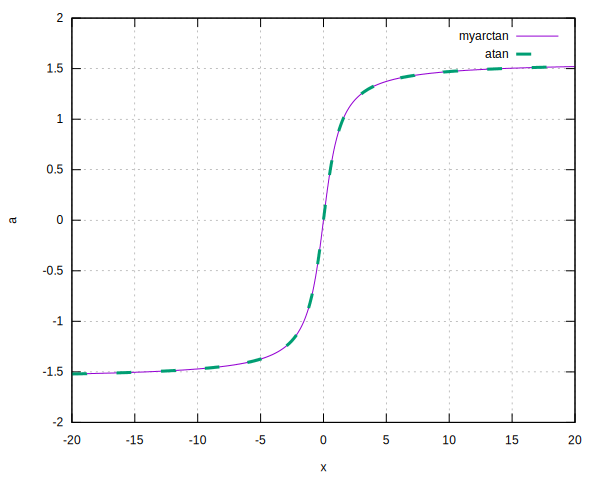
\includegraphics{plot.pdf}
	\caption{Numerical and analytical representations of the error function.}
	\label{fig:plot}
\end{figure}

\end{document}
